\documentclass[czech]{article}

\usepackage{amsmath}
\usepackage{amsfonts}
\usepackage{graphicx}
\usepackage{geometry}[margin={1cm, 2cm}]
\usepackage{babel}
\usepackage{hyperref}
\hypersetup{
    colorlinks=true,
    linkcolor=blue,
    filecolor=magenta,      
    urlcolor=cyan
    }

\title{Generativní adversariální sítě v počítačové grafice}
\author{Pavel Jakš}

\begin{document}

\selectlanguage{czech}

\maketitle

\section*{Úvod}

Jedním z moderních přístupů umělé inteligence ke generování grafického obsahu jsou tzv. \emph{generativní adversariální sítě}
(angl. \emph{generative adversarial networks}).
Jedná se o přístup ke generování obsahu pomocí dvou vzájemně nepřátelských (adversariálních) neuronových sítí,
které jsou propojeny účelovou funkcí.
Učení jedné sítě potom spočívá v minimalizaci oné účelové funkce a učení druhé sítě spočívá naopak v maximalizaci oné účelové funkce.

Zároveň první z oněch dvou neuronových sítí se nazývá generátor, neboť jejím úkolem je na základě vstupu,
kterým bývá několika dimenzionální šum (tzv. prvek latentního prostoru),
vytvořit výstup podobný vzorkům, o jejichž generování je zájem.

Druhá síť se potom nazývá diskriminátor, neboť jejím úkolem je klasifikovat, zda daný vzorek,
který je jí předložen jako vstup, pochází z generátoru či nikoliv.

Postupně se tak tyto dvě sítě společně učí, až nakonec je generátor schopen mapovat latentní prostor, tedy obyčejný šum,
na nové vzorky podobné vzorků trénovací datové sady, jejíž vzorky má generátor za cíl napodobit.

\section{Matematická formulace}

Abychom mohli formulovat problém matematicky formálně označme generátor jako funkci z latentního prostoru do prostoru vzorků:
\begin{equation}
    G_{\theta_g} : \mathbb{R}^l \rightarrow \mathbb{R}^n,
\end{equation}
kde $\theta_g$ jsou parametry generátoru jakožto neuronové sítě, $l$ je dimenze latentního prostoru a $n$ je dimenze vzorků.
Dále označme diskriminátor:
\begin{equation}
    D_{\theta_d} : \mathbb{R}^n \rightarrow (0,1),
\end{equation}
kde $\theta_d$ jsou parametry diskriminátoru jakožto neuronové sítě.
Význam působení diskriminátoru na vzorek je následující:
Pro $D_{\theta_d}(x) < 0.5$ je $x$ klasifikováno jako výsledek generátoru,
pro $D_{\theta_d}(x) >= 0.5$ je $x$ klasifikován naopak.
Potom mějme trénovací datovou sadu $\mathbb{X}$ a k ní příslušnou distribuci, která vzorky generuje $p_{data}$.
Dále mějme pravděpodobnostní rozdělení $p_l$ na latentním prostoru.

Pak lze uční generativních adversariálních sítí formulovat jako následující optimalizační problém \cite{originalpaper}:
\begin{equation} \label{optim}
    \min_{\theta_g} \max_{\theta_d} \mathbb{E}_{x \sim p_{data}(x)} \left[\operatorname{ln} D_{\theta_d} (x)\right]
    + \mathbb{E}_{z \sim p_l(z)} \left[\operatorname{ln} \left(1 - D_{\theta_d}(G_{\theta_g}(z))\right)\right].
\end{equation}

\section{Nástrahy pro implementaci}

Bohužel při implementaci učení pomocí výše napsané účelové funkce lze narazit na několik problémů.

\subsection{Nepatrný gradient}

Přístup v (\ref{optim}) je nakloněn k tomu, že v první fázi učení je gradient účelové funkce dle parametrů generátoru velmi malý,
proto se v praxi užívá přístup, že pro učení generátoru se užívá maximalizace tohoto členu:
\begin{equation}
    \mathbb{E}_{z \sim p_l(z)} \left[\operatorname{ln} D_{\theta_d}\left(G_{\theta_g}(z)\right)\right].
\end{equation}

\subsection{Kolaps módů}

Další nepříjemností, kterou generativní sítě provází, je tzv. \emph{kolaps módů} (z angl. \emph{mode collapse}).
Jedná se o stav generátoru, kdy generátor umí vytvořit pouze jeden jediný vzorek.
Pomocí proti kolapsu módů může být užití \emph{Wassersteinovy ztrátové funkce} \cite{wgan}.
Ta spočívá v nahrazení discriminátoru tzv. \emph{kritikem}.
Ten je svou podstatou opět neuronová síť, jen se nejedná o klasifikátor, zda je vzorek podvržený, či nikoliv,
nýbrž o jakéhosi hodnotitele - snaží se dát podvrženým vzorkům co nejmenší skóre a těm skutečným co největší skóre.
Potom učení kritika je řešením následujícího problému:
\begin{equation}
    \max_{\theta_k} \left\{\mathbb{E}_{x \sim p_{data}(x)} \left[K_{\theta_k} (x)\right]
    - \mathbb{E}_{z \sim p_l(z)} \left[K_{\theta_k}\left(G_{\theta_g}(z)\right)\right]\right\},
\end{equation}
kde $K_{\theta_k}$ je kritik se svými parametry $\theta_k$.
Učení generátoru je potom následující problém:
\begin{equation}
    \max_{\theta_g} \left\{ \mathbb{E}_{z \sim p_l(z)} \left[K_{\theta_k}\left(G_{\theta_g}(z)\right)\right]\right\}.
\end{equation}

Dalším úskokem od kolapsu módů může být penalizace generátoru za nízkou standardní odchylku mezi vzorky vygenerovanými v rámci jedné dávky.
Potom by při užití Wassersteinovy ztráty mohl problém generátoru vypadat následovně:
\begin{equation}
    \max_{\theta_g} \left\{ \mathbb{E}_{z \sim p_l(z)} \left[K_{\theta_k}\left(G_{\theta_g}(z)\right)\right]
     + \lambda \cdot \sum_{i = 1}^{n} \operatorname{Var}_{z \sim p_l(z)} \left[G_{\theta_g}(z)_i\right]\right\},
\end{equation}
kde $\lambda$ je vhodně zvolený hyperparametr.

\section{Výsledky}

Na datové sadě MNIST \cite{MNIST} byly natrénovány generativní adversariální sítě pomocí Wassersteinovy ztrátové funkce
a výše zmíněné regularizace.
Implementační detaily lze vyčíst ze souboru \href{https://github.com/pavel-jaks/gans/blob/main/code/J-GAN.ipynb}{J-GAN.ipynb}.
Na výsledně vygenerované obrázky po $100$ epochách učení lze nahlédnout v Obr. (\ref{obr}).

\begin{figure}
    \centering
    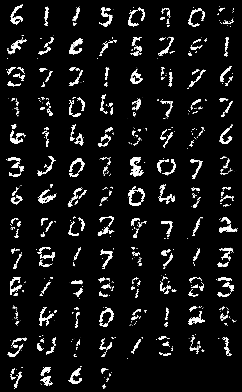
\includegraphics{graphics/samples_100.png}
    \caption{Vygenerované obrázky po $100$ epochách učení}
    \label{obr}
\end{figure}

\section*{Závěr}

Generativní adversariální sítě nabízí možnost, jak neuronovou síť naučit generovat obsah na zákadě dané datové sady.
Je třeba mít ovšem na paměti, že se jedná o velice nestabilní záležitost, která pro lazení hyperparametrů vyžaduje mnoho trpělivosti.

\newpage{}

\begin{thebibliography}{1}

\bibitem{originalpaper} I. Goodfellow, J. Pouget-Abadie, M. Mirza, B. Xu, D. Warde-Farley, S. Ozair, A. Courville, Y. Bengio,
\emph{Generative Adversarial Nets}.
Proceedings of the International Conference on Neural Information Processing Systems (NIPS 2014).

\bibitem{wgan} M. Arjovsky, S. Chintala, L. Bottou,
\emph{Wasserstein GAN}.
arXiv 2017.

\bibitem{MNIST} Y. Lecun, C. Cortes, C. J. Burges,
\emph{The mnist database of handwritten digits}. 1998.

\end{thebibliography}

\end{document}
